%========================================================================
\section{Numerical Method}\label{chap:advection-pwconst}
%========================================================================


%========================================================================
\subsection{The Base Update Formula}
%========================================================================

\begin{figure}[htbp]
	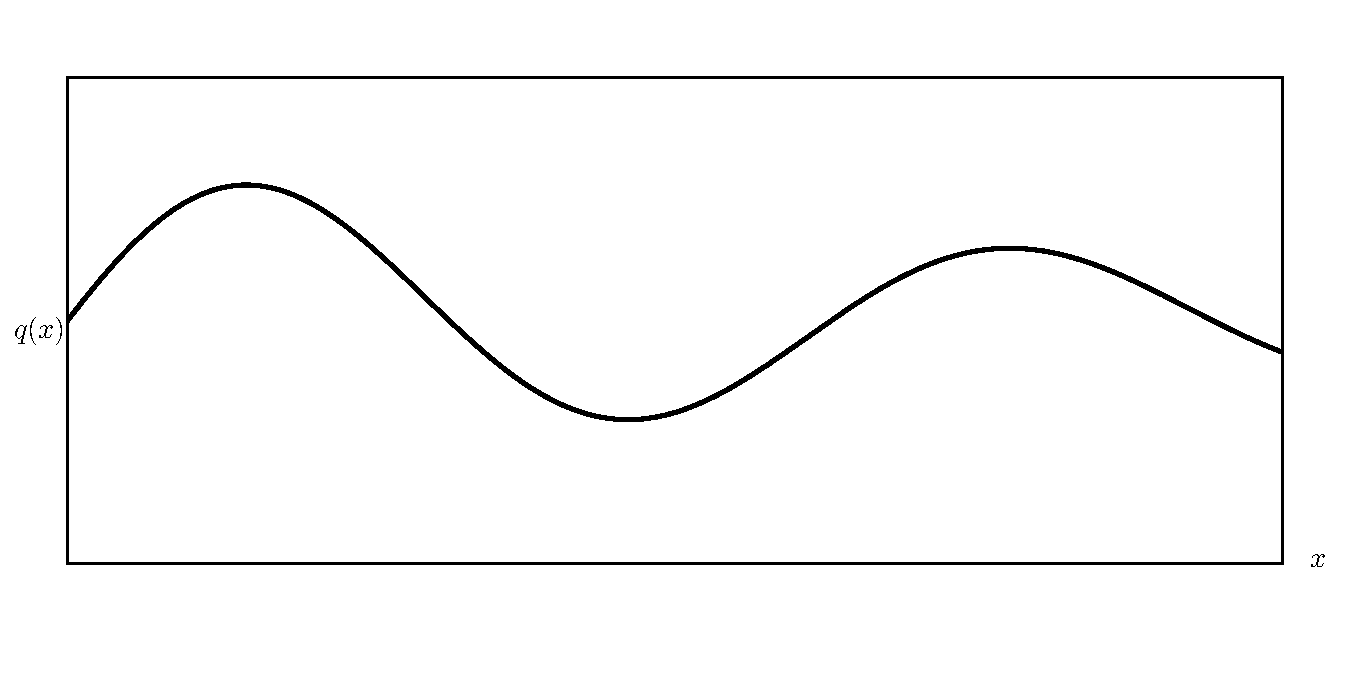
\includegraphics[width=.9\textwidth]{./figures/q_of_x.pdf}\\%
	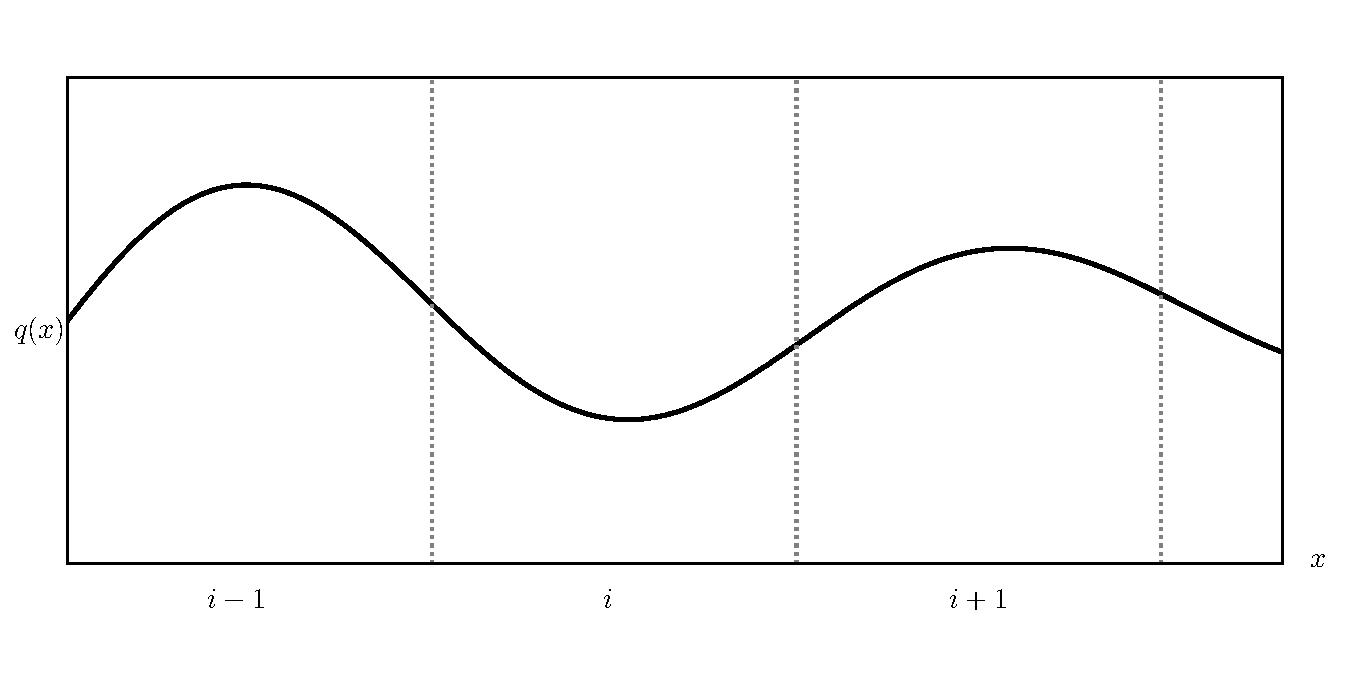
\includegraphics[width=.9\textwidth]{./figures/adding_cells.pdf}\\%
	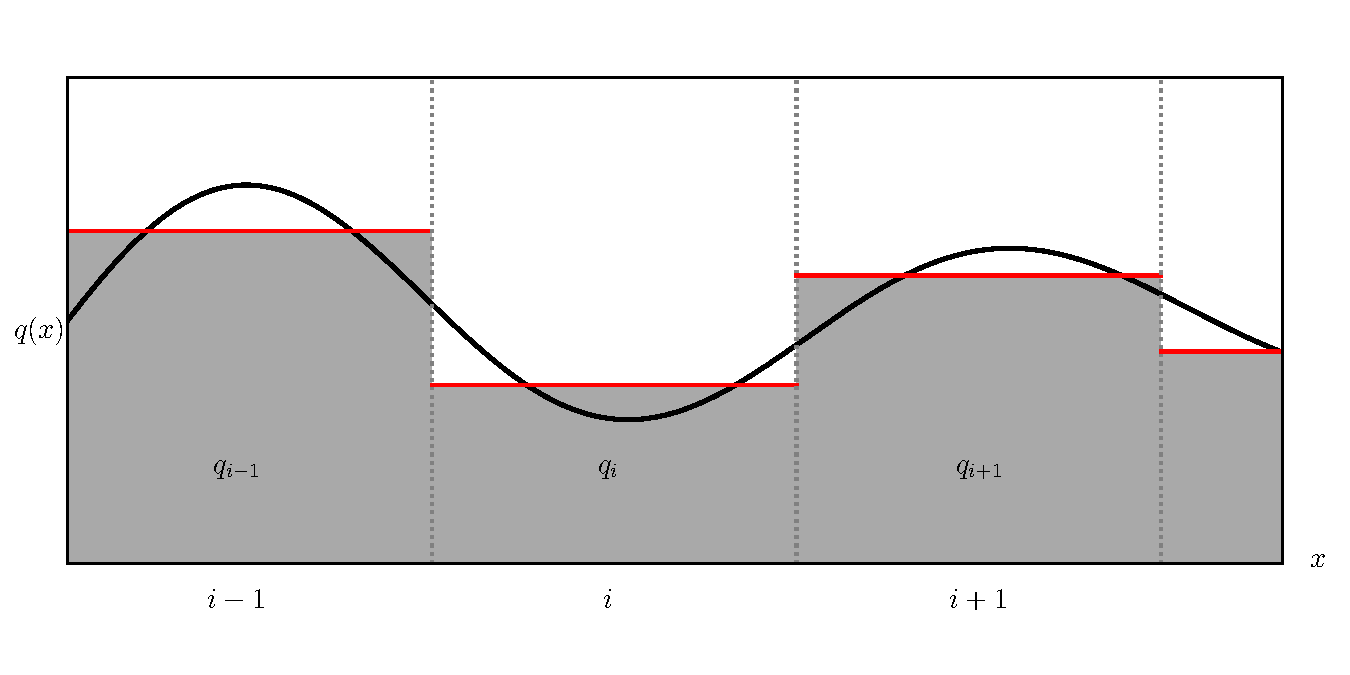
\includegraphics[width=.9\textwidth]{./figures/piecewise_const.pdf}%
	\caption{
		Piecewise constant reconstruction of the field. We start with some function
		$q(x)$ (top row). Then we introduce cells with equal spacings $\Delta x$ and
		indexes $i - 1$, $i$, and $i + 1$ (middle row). Finally, we average the
		initial quantity $q(x)$ inside each cell to obtain that cell's discretized
		value $q_i$, assuming that the states within each cell are constant.
	}
	\label{fig:pwconst}
\end{figure}


First things first: We need to discretize the problem. To do so, we use a very
simple approach for this exercise, where we replace the analytical derivatives
with approximate discrete ones.

But before we can do that, we need to define a discrete version of our initial
problem. Suppose you split the domain you want to simulate into $N$ cells of
equal sizes $\Delta x$. Let each cell have an index $i$.
% Then the interfaces of
% cell $i$ with neighbouring cells $i - 1$ and $i + 1$ are given with indexes
% $i - \half$ and $i + \half$, respectively.

We assume that a state $q$ is constant within a cell. See Figure~\ref{fig:pwconst}
for a visual representation. This approach is called ``piecewise constant reconstruction''.

Suppose we're solving the equation over some small time step size $\Delta t$, and
that each cell has the same size $\Delta x$. We can now replace the analytical
derivatives with discrete ones:

\begin{align}
	\deldt{q(x_i, t)} &\approx \frac{q(x_i, t + \Delta t) - q(x_i, t)}{\Delta t} \\
	\deldx{q(x_i, t)} &\approx \frac{q(x_i, t) - q(x_i - \Delta x, t)}{\Delta x} \label{eq:approx-gradient}
\end{align}

Using the notation

\begin{align}
	q(x_i) &= q_i \\
	q(x_i - \Delta x) &= q_{i-1} \\
	q(t) &= q^n \\
	q(t + \Delta t) &= q^{n + 1}
\end{align}

we arrive at the update formula:

\begin{equation}
\boxed{
	q_i^{n+1} = q_i^{n} +  a \frac{\Delta t}{\Delta x} \left( q_{i-1}^n - q_{i}^n \right)
}
\label{eq:advection-first-order}
\end{equation}



Note that we also assume that the advection velocity, $a$, is also constant and positive.
If it were negative, we'd need to modify our expression for the approximate gradient in
eq.~\ref{eq:approx-gradient}.\footnote{
	If $a$ were negative, we'd have to modify our gradient as $\deldx{q_i} \approx \frac{q_{i+1} - q_i}{\Delta x}$.
	The important point is that we always do \emph{upwind differencing}. To obtain a
	finite difference, as we do here, you must never use the value that is downstream,
	i.e. that is in the direction of the flux, or the flow. Doing that means you'd be
	taking a value for your computation that won't be valid as soon as an infinitesimal
	time interval passes, because the ingoing flux will change the downwind state.
	This is unphysical and leads to violent instabilities.
}









%====================================================
\subsection{The CFL Condition}
%====================================================

In our derivation of the numerical method above we simply assumed that the time
step size $\Delta t$ is sufficiently small. But how small is ``sufficient''?

The restriction of a maximal time step size is given by the so-called
Courant-Friedrichs-Levy condition (CFL condition). In principle, that condition
is derived through analysis of the numerical method with regards to stability and
accuracy. In practice, an intuitive explanation is readily available for the one-dimensional
case, which luckily is what we're trying to solve.

Note how in our approximate gradient expression (eq.~\ref{eq:approx-gradient})
we only used values of an adjacent cell with index $i - 1$. So what would happen if
we let the quantity be advected more than a cell width during a single time step, i.e.
if the quantity gets advected to two, three, four cells away downstream? The answer is -
undefined, unphysical behavior. Our method is not set up to account for changes that
occur further away than a single cell width next to it. Therefore, we must limit the
time step size such that the quantity never gets advected further than a single cell width
during a single time step size. In other words, we must enforce:

\begin{equation}
	a \cdot \Delta t_{max} \leq \Delta x
\end{equation}

This condition is typically written as:

\begin{equation}
	\Delta t_{max} = C_{cfl} \frac{\Delta x}{a} \label{eq:CFL1D}
\end{equation}

with $C_{cfl} \in [0, 1) $ a user-set factor.
The lower it is, the more accurate the results, but the more computations
(i.e. time steps) you need to do to complete your simulation.






%======================================================================
\subsection{Boundary Conditions}\label{chap:boundary-conditions}
%======================================================================


\begin{figure}[htbp]
	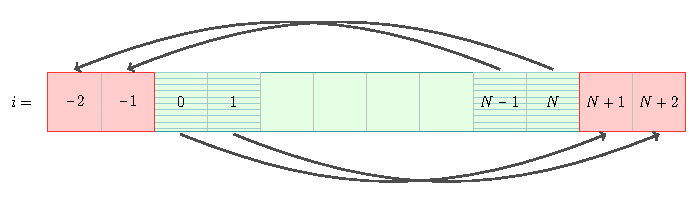
\includegraphics[width=\textwidth]{./figures/boundary_periodic.pdf}%
	\caption{\label{fig:boundary_periodic}
		Method to obtain periodic boundary conditions.
		The ghost cells are red, the arrows show what will be copied where.
	}
\end{figure}



For this exercise, we employ \emph{periodic boundary conditions}. Basically this means
that we set up the solver such that whatever leaves or enters on one side of our simulation
box, enters or leaves on the opposite side, respectively.

To achieve this behavior, we add additional cells (``\emph{ghost cells}'') around our simulation box.
How many cells you need to add depends on the methods (and mostly stencils) you use.
If you only take into account one neighboring cell, then one ghost cell on every boundary suffices.
(This is the case that we're working with.)
In Figure~\ref{fig:boundary_periodic}, two such ghost cells for a 1D grid are drawn.

Suppose we have 1D grid with $N$ cells and require 2 ghost cells each, which will have indices $-2$, $-1$, $N+1$, and $N+2$.
We obtain periodic boundary conditions by enforcing

\begin{align*}
	q_{-2} &= q_{N-1} \\
	q_{-1} &= q_{N}	\\
	q_{N+1} &= q_0 	\\
	q_{N+2} &= q_1
\end{align*}





%==============================================
\subsection{The Full Algorithm}
%==============================================

Finally, a brief description of the full algorithm of the solver.

To start, set $t_{current} = t^0 = t_{start}$ and set up the initial states $q_i^0$ for
each cell $i$.\\[.5em]
%
While $t_{current} < t_{end}$, solve the $n$-th time step:\\[.5em]
%
\indent~~~~Find the maximal permissible time step $\Delta t$ using eq.~\ref{eq:CFL1D} \\[.5em]
%
\indent~~~~Apply the periodic boundary conditions \\[.5em]
%
\indent~~~~For each cell $i$, find the updated states $q_i^{n+1}$ using
eq.~\ref{eq:advection-first-order-overview} \\[.5em]
%
\indent~~~~Update the current time: $t_{current} = t^{n+1} = t^n + \Delta t$


